\section{Konventionelle Abhängigkeitsanalyse} % (fold)
\label{sec:konventionelle_abhaengigkeitsanalyse}
\subsubsection{Prinzipielles Vorgehen am Beispiel} % (fold)
\label{ssub:prinzipielles_vorgehen_am_beispiel}

\begin{itemize}
    \item synthetisierte Atribute für Zuweisungen im Parsebaum
    \begin{itemize}
        \item gen[S]: die Definitionen eines Statements S
        \item kill[S]: solche Definitionen, die von Statement S überschrieben werden
    \end{itemize}
    \item Verallgemeinerung auf zusammengesetzte Anweisungen und auf Mengen von Anweisungen, insbesondere auf \glqq basic blocks\grqq
    \item Berechnung entlang des Syntaxbaums (bottom-up) durch \emph{Datenflussgleichungen} -- oder allgemein durch Fixpunktiteration.
\end{itemize}



\paragraph{zusammengesetzte Anweisungen} % (fold)
\label{par:zusammengesetzte_anweisungen}
Verallgemeinerung von gen[S] und kill[S] auf zusammengesetzte Anwesungen wie Sequenz, Konditional und Schleife.\\
Daher ist eine Abschätzung notwendig:
\begin{itemize}
    \item gen legt fest: es könnte generiert worden sein.
    \item kill bedeutet, es ist garantiert gelöscht worden.
\end{itemize}

Die Berechnung erfolgt entlang des Parsebaums (bootom-up) durch \emph{Datenflussgleichungen}.
% paragraph zusammengesetzte_anweisungen (end)

% subsubsection prinzipielles_vorgehen_am_beispiel (end)

\subsubsection{Datenflussgleichungen} % (fold)
\label{ssub:datenflussgleichungen}

\begin{figure}[!ht]
    \centering
    % 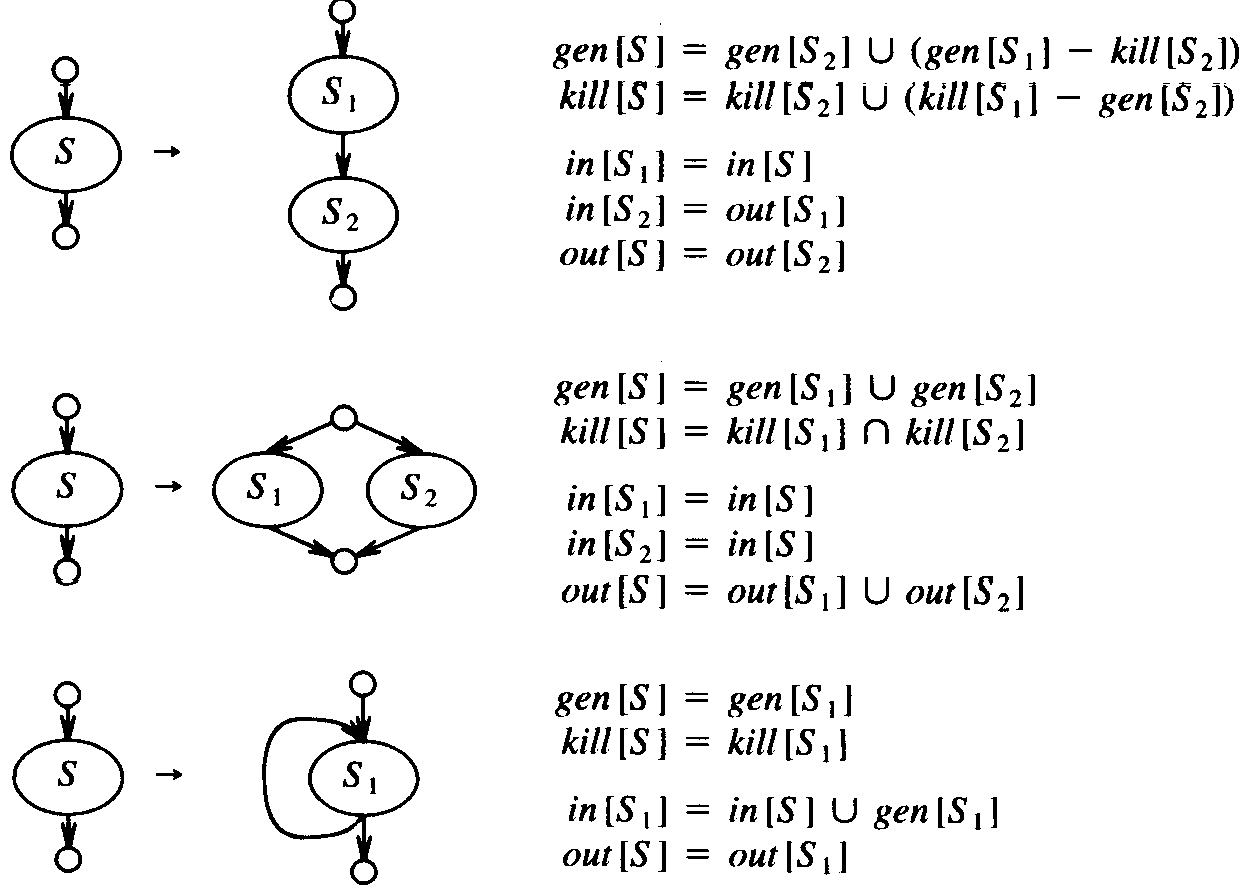
\includegraphics[scale=0.2]{images/bild0-2.png}
    \includegraphics[scale=0.2]{images/b02.epsi}
    \caption{Datenflussgleichungen für zusammengesetzte Anweisungen}
\end{figure}

\begin{figure}[!ht]
    \centering
    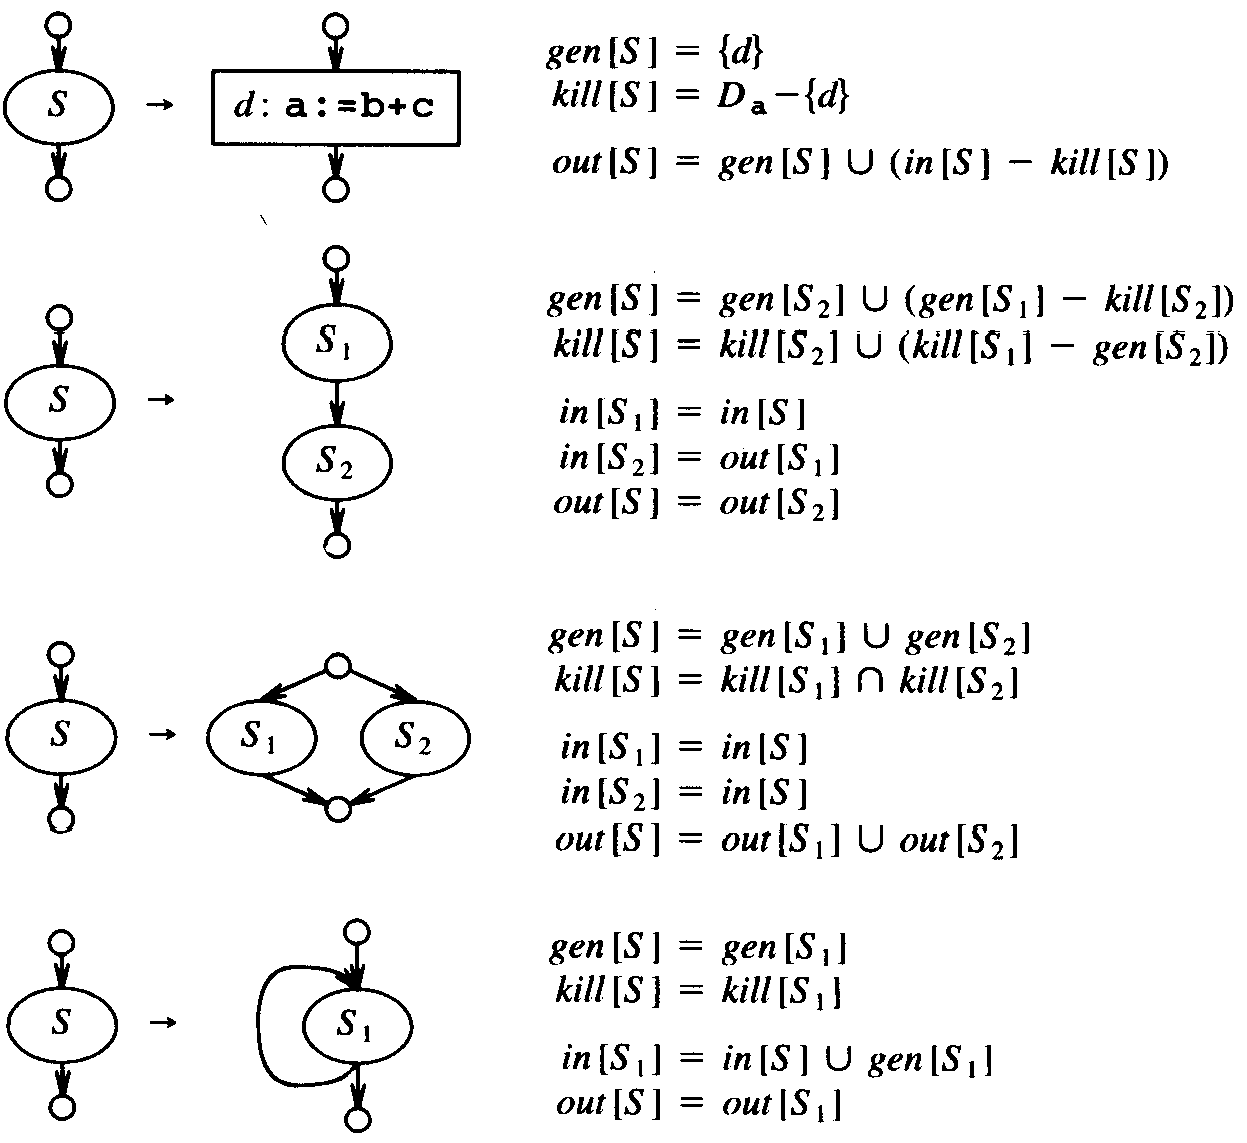
\includegraphics[scale=0.2]{images/bild1-3.png}
    \caption{Datenflussgleichungen für \glqq erreichende Definitionen\grqq\ }
\end{figure}

% subsubsection datenflussgleichungen (end)
\newpage
\subsubsection{Beispielprogramm} % (fold)
\label{ssub:beispielprogramm}
~\\
\begin{figure}[!ht]
    \centering
    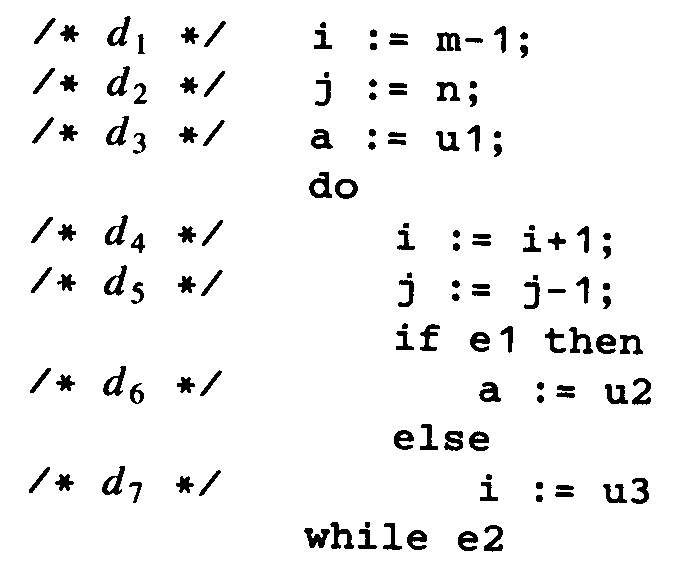
\includegraphics[scale=0.2]{images/bild3-1.png}
    \caption{Beispielprogramm}
\end{figure}
% subsubsection beispielprogramm (end)

\newpage

\subsubsection{Resultat} % (fold)
\label{ssub:resultat}
~\\
\begin{figure}[!ht]
    \centering
    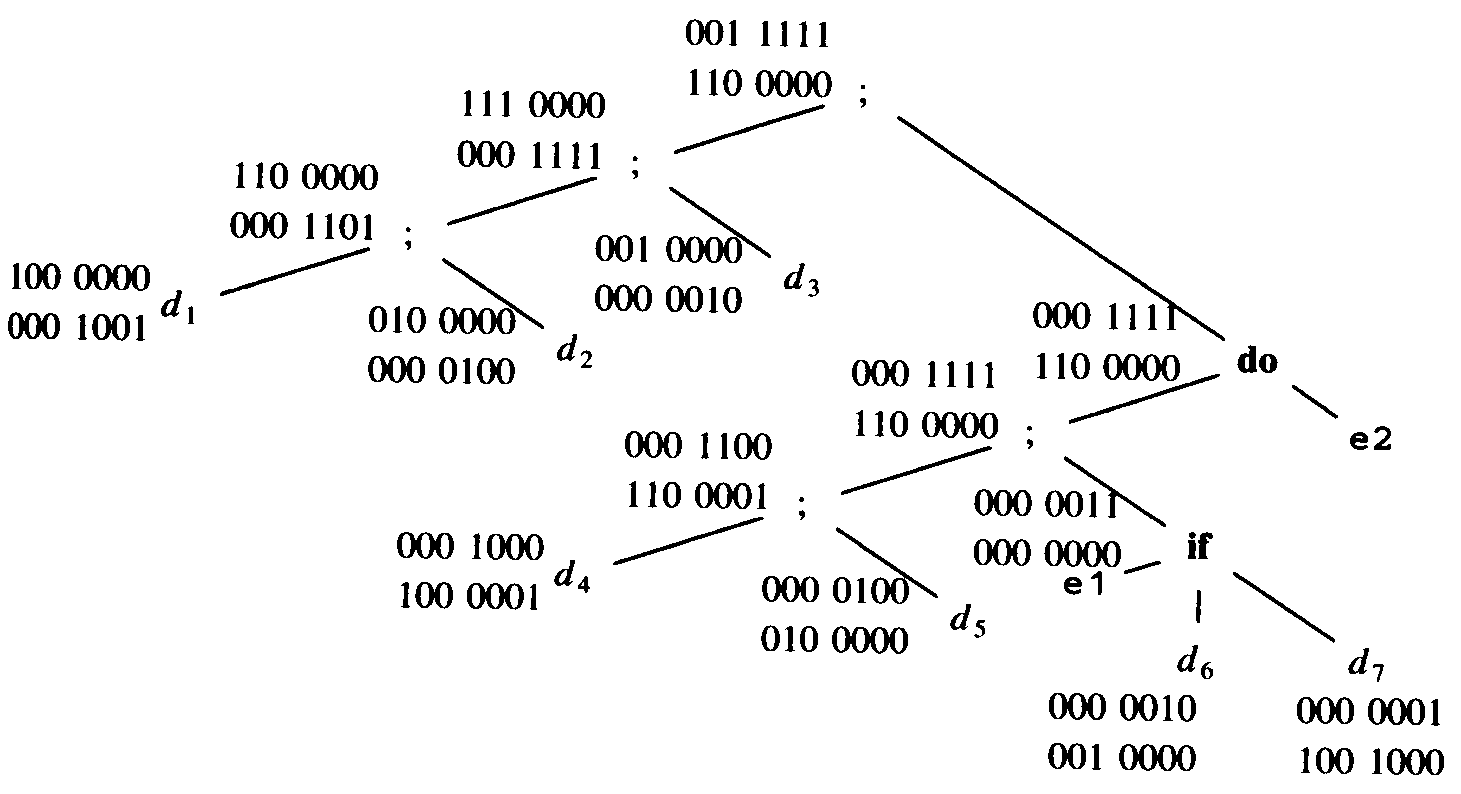
\includegraphics[scale=0.2]{images/bild2-1.png}
    \caption{Resultat}
\end{figure}

% subsubsection resultat (end)

\subsubsection{Nachteile dieses Verfahrens} % (fold)
\label{ssub:nachteile_dieses_verfahrens}
\begin{itemize}
    \item Bitvektor-Darstellung ungeeignet für Arrays
    \item Konflikte, z.\,B. für kill, nur ungenau:
    \begin{itemize}
        \item auf Variablennamen basiert (für Array ungeeignet)
        \item keine Berücksichtigung von eventuell bekannten Schleifengrenzen
        \item keine Berücksichtigung der sequentiellen Ausführungsordnung
    \end{itemize}
    \item für jedes Analyseziel ein neues Datenflussgleichungssystem von Grund auf neu berechnen
    \item im allgemeinen Fall Fixpunktiteration nötig
\end{itemize}
% subsubsection nachteile_dieses_verfahrens (end)
% section konventionelle_abhaengigkeitsanalyse (end)
